\documentclass[13pt,oneside]{book}
\usepackage[utf8]{inputenc}
\usepackage{url}
\usepackage{graphicx}

\usepackage{geometry}
\geometry{a4paper, left=20mm, right=20mm, top=20mm, bottom=20mm}
\usepackage[margin=1.2in]{geometry}
\usepackage[toc,page]{appendix}
\usepackage{graphicx}
\usepackage{natbib}
\usepackage{lipsum}
\usepackage{caption}

\begin{document}

\captionsetup[figure]{margin=1.5cm,font=small,labelfont={bf},name={Figure},labelsep=colon,textfont={it}}
\captionsetup[table]{margin=1.5cm,font=small,labelfont={bf},name={Table},labelsep=colon,textfont={it}}
\setlipsumdefault{1}

\begin{titlepage}
\begin{center}
{\LARGE College Of Engineering Trivandrum}\\[3cm]
\linespread{1.2}\huge {\bfseries Application Software Development Lab}\\[3cm]
\linespread{1}

\includegraphics[width=5cm]{img/emblem.jpeg}\\[3cm]
{\Large GOKUL K\\ S5  CSE \\ Roll No:21\\ TVE18CS021 }\\[1cm]


\textit{ }\\[2cm]
Department of Computer Science\\[0.2cm]
\today
\end{center}

\end{titlepage}

\newpage

\begin{frame}{}
    \centering
    \hspace*{-0.5cm}
    $\vcenter{\hbox{
\includegraphics[width=1.5cm]{img/emblem.jpeg}}}$
    $\vcenter{\resizebox{0.95\textwidth}{!}{
        \begin{tabular}{c}
             CS333 - Application Software Development Lab $\cdot$ 2020 $\cdot$   \\
             \hline 
        \end{tabular}
    }}$
\end{frame}
\section*{Cycle 1}
\section*{Expt 7}
\begin{center}
    \Large{JOIN STATEMENTS, SET OPERATIONS, NESTED QUERIES AND GROUPING}
\end{center}

\section*{Aim}
\large To get introduced to:\\
a) UNION\\
b) JOIN\\
c) INTERSECTION\\
d) NESTED QUERIES\\
e) MINUS\\
f) GROUP BY \& HAVING\\

\section*{Expiriment}
\begin{itemize}
	\item
	Create Items, Orders, Customers, Delivery tables, populate them with appropriate data
	 and display the tables.
	 
	Syntax:
	\begin{verbatim}
	CREATE TABLE Items (
			itemid INT PRIMARY KEY,
			itemname VARCHAR(50),
			category VARCHAR(20),
			price INT,
			instock INT
	);
	CREATE TABLE Customers (
			custid INT PRIMARY KEY,
			custname VARCHAR(20),
			address VARCHAR(40),
			state VARCHAR(20)
	);
	CREATE TABLE Orders (
			orderid INT PRIMARY KEY,
			itemid INT,
			quantity INT NOT NULL,
			orderdate DATE,
			custid INT,
			FOREIGN KEY (itemid) REFERENCES Items(itemid) ON UPDATE CASCADE ON DELETE CASCADE,
			FOREIGN KEY (custid) REFERENCES Customers(custid) ON UPDATE CASCADE ON DELETE CASCADE 
	);
	CREATE TABLE Delivery (
			deliveryid INT PRIMARY KEY,
			orderid INT,
			custid INT,
			FOREIGN KEY (orderid) REFERENCES Orders(orderid) ON UPDATE CASCADE ON DELETE CASCADE,
			FOREIGN KEY (custid) REFERENCES Customers(custid) ON UPDATE CASCADE ON DELETE CASCADE 
	);
	INSERT INTO Items
	VALUES
			(5,'sony z5 premium','electronics',5005,1),
			(4,'Samsung Galaxy S4','electronics',5005,1),
			(3,'One Plus 7','electronics',6006,2),
			(2,'Iphone X','electronics',7007,6),
			(1,'Xiomi','electronics',1001,6);
	INSERT INTO Customers
	VALUES
			(111,'elvin','202 jai street','delhi'),
			(113,'soman','puthumana','kerala'),
			(115,'mickey','juhu','maharastra'),
			(112,'patrick','harinagar','tamilnadu'),
			(114,'jaise','kottarakara','kerala');
	INSERT INTO Orders
	VALUES
			(1,1,2,'2014-10-11',111),
			(2,3,1,'2012-01-29',113),
			(3,5,1,'2013-05-13',115),
			(4,4,3,'2014-12-22',114);
	INSERT INTO Delivery
	VALUES
			(1001,1,111),
			(1002,2,113),
			(1003,3,115);
	SELECT * FROM Items;
	SELECT * FROM Customers;
	SELECT * FROM Orders;
	SELECT * FROM Delivery;
	
	\end{verbatim}
	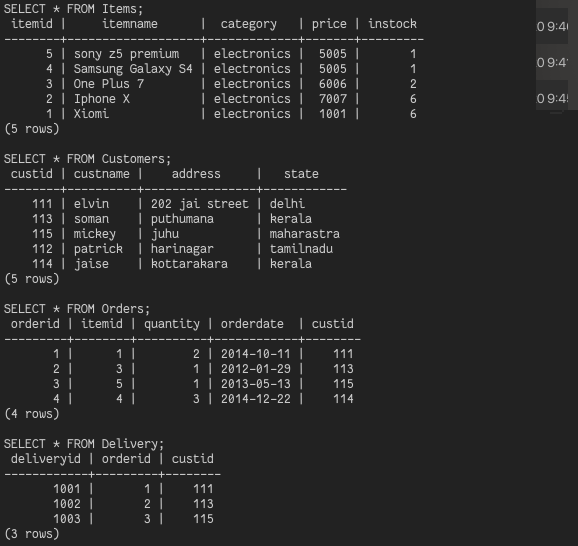
\includegraphics[]{img/p7/ss1.png}
	
	
	\item
	List the details of all customers who have placed an order.
	 
	Syntax:
	\begin{verbatim}
	SELECT Customers.custid,custname,address,state FROM Customers, Orders
	WHERE Orders.custid = Customers.custid;
	
	\end{verbatim}
	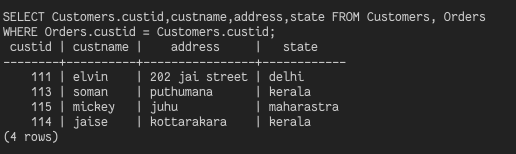
\includegraphics[]{img/p7/ss2.png}
	
	
	\item
	List the details of all customers whose orders have been delivered
	 
	Syntax:
	\begin{verbatim}
	SELECT Customers.custid, custname, address, state FROM Customers, Delivery
	WHERE Delivery.custid = Customers.custid;
	
	\end{verbatim}
	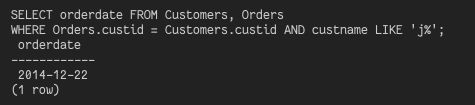
\includegraphics[]{img/p7/ss3.png}
	
	
	\item
	Find the orderdate for all customers whose name starts in the letter 'J'
	 
	Syntax:
	\begin{verbatim}
	SELECT orderdate FROM Customers, Orders
	WHERE Orders.custid = Customers.custid AND custname LIKE 'j%';
	
	\end{verbatim}
	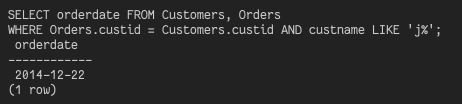
\includegraphics[]{img/p7/ss4.png}
	
	
	\item
	Display the name and price of all items bought by the customer 'Mickey'
	 
	Syntax:
	\begin{verbatim}
	SELECT itemname, price FROM Items AS i, Customers AS c, Orders AS o
	WHERE i.itemid = o.itemid and c.custid = o.custid AND c.custname LIKE 'mickey';
	
	\end{verbatim}
	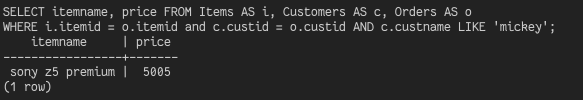
\includegraphics[]{img/p7/ss5.png}
	
	
	\item
	List the details of all customers who have placed an order after January 2013 and not
	 received delivery of items.
	 
	Syntax:
	\begin{verbatim}
	SELECT c.* FROM Customers AS c, Orders AS o
	WHERE o.custid = c.custid AND orderdate >= '2013-01-01' AND 
			c.custid NOT IN (SELECT custid FROM Delivery);
	
	\end{verbatim}
	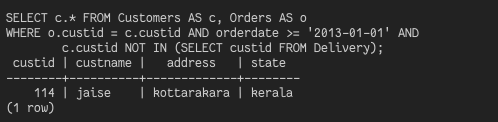
\includegraphics[]{img/p7/ss6.png}
	
	
	\item
	Find the itemid of items which has either been ordered or not delivered. (Use SET
	 UNION)
	 
	Syntax:
	\begin{verbatim}
	(SELECT i.itemid FROM Items AS i, Orders AS o
	WHERE i.itemid = o.itemid)
			UNION
	(SELECT i.itemid from Items AS i, Orders AS o
	WHERE i.itemid = o.itemid AND o.orderid NOT IN
			(SELECT orderid FROM Delivery));
	
	\end{verbatim}
	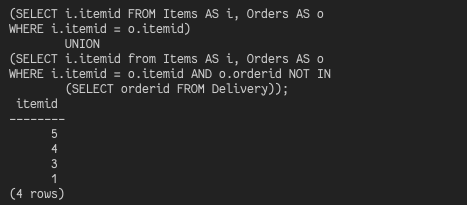
\includegraphics[]{img/p7/ss7.png}
	
	
	\item
	Find the name of all customers who have placed an order and have their orders
	 delivered.(Use SET INTERSECTION)
	 
	Syntax:
	\begin{verbatim}
	(SELECT custname FROM Customers AS c, Orders AS o
	WHERE o.custid = c.custid)
			INTERSECT
	(SELECT custname FROM Customers AS c, Delivery AS d
	WHERE d.custid = c.custid);
	
	\end{verbatim}
	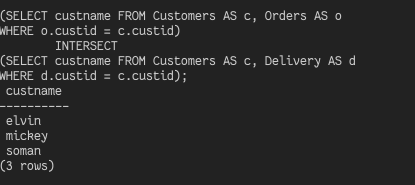
\includegraphics[]{img/p7/ss8.png}
	
	
	\item
	Find the custname of all customers who have placed an order but not having their
	 ordersdelivered. (EXCEPT is available in the PostgreSQL database while MINUS is
	 available in MySQL)
	 
	Syntax:
	\begin{verbatim}
	(SELECT custname FROM Customers AS c, Orders AS o
	WHERE o.custid = c.custid)
			EXCEPT
	(SELECT custname FROM Customers AS c, Delivery AS d 
	WHERE d.custid = c.custid);
	
	\end{verbatim}
	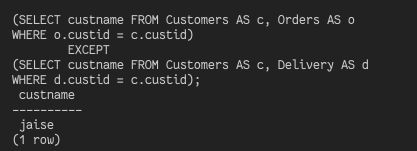
\includegraphics[]{img/p7/ss9.png}
	
	
	\item
	Find the name of the customer who has placed the most number of orders.
	 
	Syntax:
	\begin{verbatim}
	INSERT INTO Orders VALUES (5, 2, 1, '2012-05-25', 115);
	SELECT * FROM Customers WHERE custid=(
			SELECT custid FROM Orders GROUP BY custid ORDER BY COUNT(*) DESC LIMIT 1
	);
	
	\end{verbatim}
	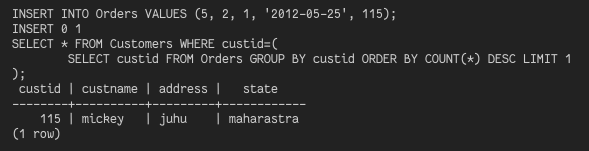
\includegraphics[]{img/p7/ss10.png}
	
	
	\item
	Find the details of all customers who have purchased items exceeding a price of
	 5000\$.
	 
	Syntax:
	\begin{verbatim}
	SELECT c.* FROM Customers AS c, Items AS i, Orders AS o
	WHERE o.itemid = i.itemid AND c.custid = o.custid AND price > 5000;
	
	\end{verbatim}
	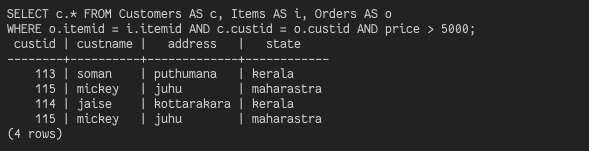
\includegraphics[]{img/p7/ss11.png}
	
	
	\item
	Find the name and address of customers who has not ordered a 'Samsung Galaxy S4'
	 
	Syntax:
	\begin{verbatim}
	(SELECT custname, address FROM Customers)
			EXCEPT
	(SELECT c.custname, c.address FROM Customers AS c, Orders as o, Items as i
	WHERE o.itemid = i.itemid AND c.custid = o.custid AND itemname = 'Samsung Galaxy S4');
	
	\end{verbatim}
	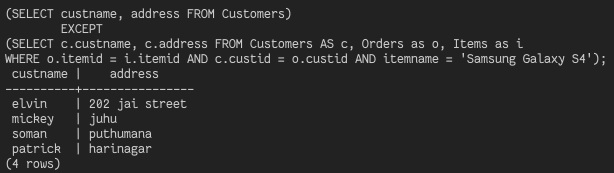
\includegraphics[]{img/p7/ss12.png}
	
	
	\item
	Perform Left Outer Join and Right Outer Join on Customers \& Orders Table.
	 
	Syntax:
	\begin{verbatim}
	SELECT * FROM Customers LEFT OUTER JOIN Orders ON Customers.custid = Orders.custid;
	SELECT * FROM Customers RIGHT OUTER JOIN Orders ON Customers.custid = Orders.custid;
	
	\end{verbatim}
	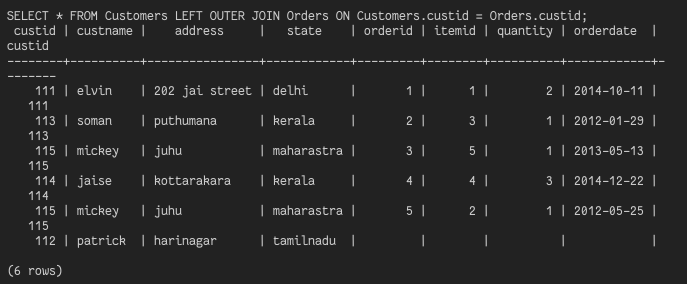
\includegraphics[]{img/p7/ss13.1.png}
	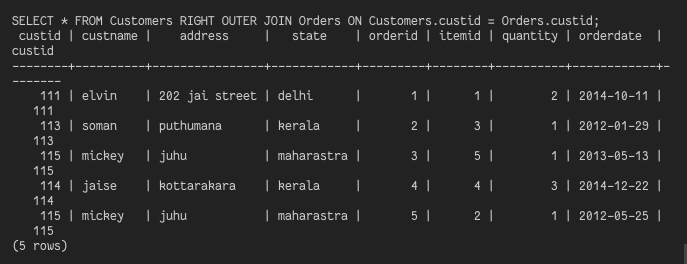
\includegraphics[]{img/p7/ss13.2.png}
	
	
	\item
	Find the details of all customers grouped by state.
	 
	Syntax:
	\begin{verbatim}
	SELECT COUNT(*), state FROM Customers 
	GROUP BY state;
	
	\end{verbatim}
	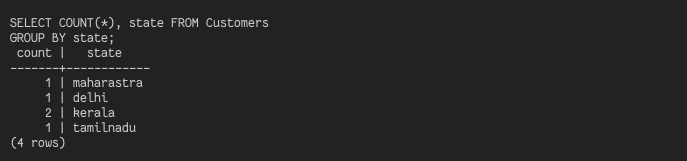
\includegraphics[]{img/p7/ss14.png}
	
	
	\item
	Display the details of all items grouped by category and having a price greater than
	 the average price of all items.
	
	Syntax:
	\begin{verbatim}
	SELECT * FROM Items
	WHERE price IN (
			SELECT price FROM Items
			GROUP BY price
			HAVING price > (
					SELECT AVG(price) FROM Items
					GROUP BY category
			)
	);
	\end{verbatim}
	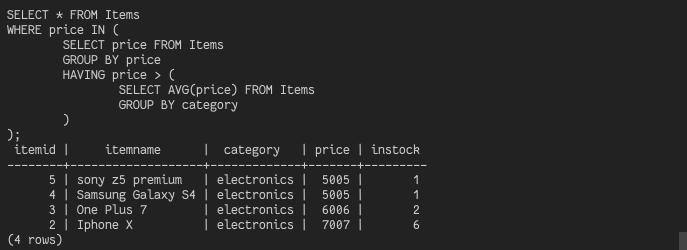
\includegraphics[]{img/p7/ss15.png}
	
\end{itemize}
\section*{Result}
	The basic SQL for creating and modifying a table is executed and their output
	is verified in a PostgreSQL environment.
\end{document}